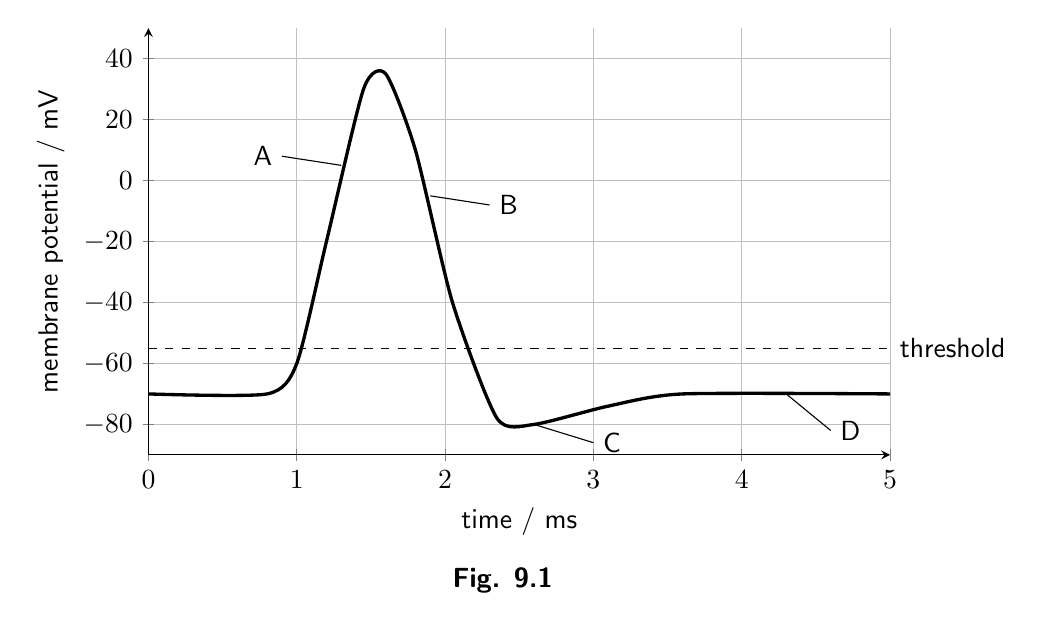
\begin{tikzpicture}[font=\sffamily]
  \begin{axis}[
    width=11cm, height=7cm, clip=false,
    axis lines=left, xmin=0, xmax=5, ymin=-90, ymax=50,
    xtick={0,...,5}, ytick={-80,-60,...,40}, grid=major,
    xlabel={time / ms}, ylabel={membrane potential / mV},
  ]
    \addplot[very thick, smooth, tension=0.4] coordinates {(0,-70) (0.8,-70) (1.0,-60) (1.2,-20) (1.45,30) (1.6,35) (1.8,10) (2.05,-40) (2.35,-78) (2.6,-80) (3.1,-74) (3.6,-70) (5,-70)};
    \draw[dashed] (axis cs:0,-55)--(axis cs:5,-55) node[right] {threshold};
    \draw (axis cs:1.3,5)--(axis cs:0.9,8) node[left] {A};
    \draw (axis cs:1.9,-5)--(axis cs:2.3,-8) node[right] {B};
    \draw (axis cs:2.6,-80)--(axis cs:3.0,-86) node[right] {C};
    \draw (axis cs:4.3,-70)--(axis cs:4.6,-82) node[right] {D};
  \end{axis}
  \node[font=\sffamily\bfseries] at (4.5,-1.6) {Fig. 9.1};
\end{tikzpicture}
